\documentclass[tikz,border=6pt]{standalone}
\usepackage[T1]{fontenc}
\usepackage{lmodern}
\usepackage{amsmath,amssymb}
\usetikzlibrary{arrows.meta,calc,positioning,shapes.geometric,patterns,decorations.pathmorphing,backgrounds,fit}
\definecolor{ink}{HTML}{173948}
\definecolor{flow}{HTML}{167D9A}
\definecolor{heat}{HTML}{B75A23}
\definecolor{measure}{HTML}{70518A}
\definecolor{pale}{HTML}{EAF2F5}
\definecolor{muted}{HTML}{526571}
\definecolor{green}{HTML}{2E8665}
\tikzset{every node/.style={font=\sffamily\small,text=ink},
 equipment/.style={draw=ink,line width=1pt,fill=pale,rounded corners=2pt},
 process/.style={draw=flow,line width=1.1pt,-{Latex[length=2.4mm]}},
 signal/.style={draw=measure,dashed,line width=.9pt,-{Latex[length=2mm]}},
 thermal/.style={draw=heat,line width=1.1pt,-{Latex[length=2.3mm]}},
 labelbox/.style={fill=white,inner sep=2pt,font=\sffamily\footnotesize,align=center},
 annotation/.style={font=\sffamily\footnotesize,text=muted,align=left},
 panel/.style={draw=ink!20,fill=ink!2,rounded corners=3pt,inner sep=7pt,align=left},
 sensor/.style={circle,draw=measure,fill=white,line width=.8pt,minimum size=8mm,inner sep=1pt,font=\sffamily\scriptsize,align=center},
 box/.style={equipment,minimum width=3cm,minimum height=1.2cm,align=center}}
\newcommand{\atlasheader}[2]{\node[anchor=north west,font=\sffamily\bfseries\LARGE]at(0,0){#1};\node[anchor=north west,font=\sffamily\small,text=muted]at(0,-.75){#2};\draw[ink!25](0,-1.25)--(26,-1.25);}
\newcommand{\atlasfooter}[1]{\draw[ink!25](0,-15.8)--(26,-15.8);\node[anchor=north west,annotation,text width=25.8cm]at(0,-16){#1\\Original explanatory drawing for ThermoFuzzy-PID. Source traceability: Cordeiro (UFC, 2021), documented repository equations and explicit reconstruction choices.};}

\begin{document}
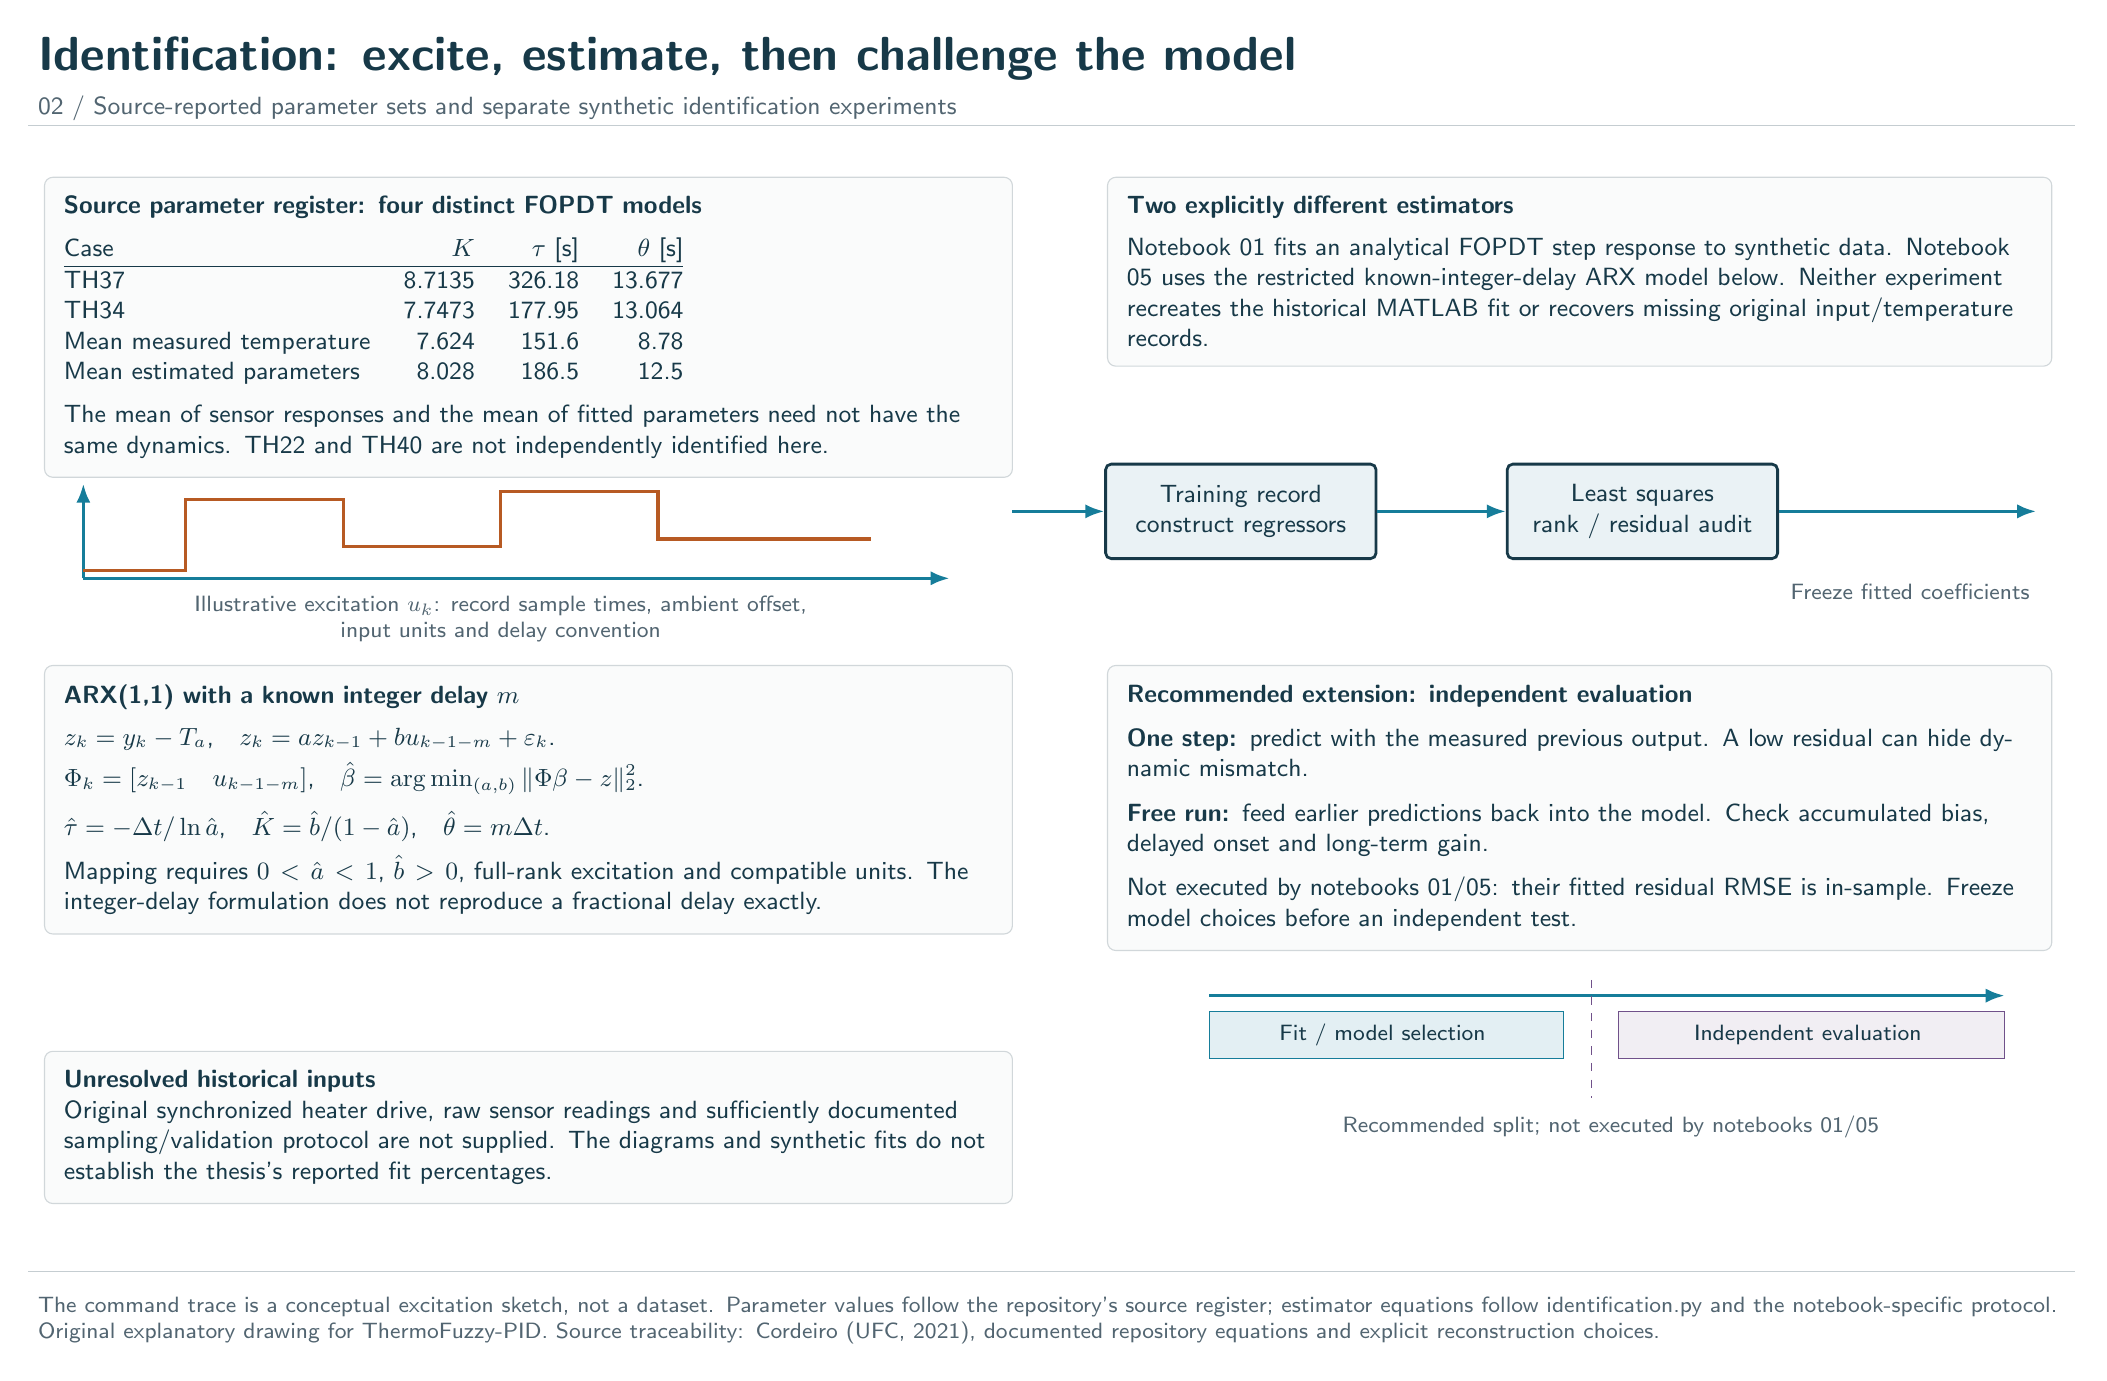
\begin{tikzpicture}[x=1cm,y=1cm]
\atlasheader{Identification: excite, estimate, then challenge the model}{02 / Source-reported parameter sets and separate synthetic identification experiments}
\node[panel,anchor=north west,text width=11.8cm]at(.2,-1.9){\textbf{Source parameter register: four distinct FOPDT models}\\[5pt]
\begin{tabular}{@{}lrrr@{}}Case & $K$ & $\tau$ [s] & $\theta$ [s]\\\hline
TH37 & 8.7135 & 326.18 & 13.677\\
TH34 & 7.7473 & 177.95 & 13.064\\
Mean measured temperature & 7.624 & 151.6 & 8.78\\
Mean estimated parameters & 8.028 & 186.5 & 12.5
\end{tabular}\\[5pt]
The mean of sensor responses and the mean of fitted parameters need not have the same dynamics. TH22 and TH40 are not independently identified here.};
\node[panel,anchor=north west,text width=11.5cm]at(13.7,-1.9){\textbf{Two explicitly different estimators}\\[4pt]
Notebook 01 fits an analytical FOPDT step response to synthetic data. Notebook 05 uses the restricted known-integer-delay ARX model below. Neither experiment recreates the historical MATLAB fit or recovers missing original input/temperature records.};
% Measured time-series contract and chronological partition.
\draw[process](.7,-7.0)--(11.7,-7.0);
\draw[process](.7,-7.0)--(.7,-5.8);
\draw[heat,line width=1.2pt](.7,-6.9)--(2,-6.9)--(2,-6.0)--(4,-6.0)--(4,-6.6)--(6,-6.6)--(6,-5.9)--(8,-5.9)--(8,-6.5)--(10.7,-6.5);
\node[annotation,anchor=north,align=center]at(6,-7.1){Illustrative excitation $u_k$: record sample times, ambient offset,\\input units and delay convention};
\node[box,text width=3.2cm] (train)at(15.4,-6.15){Training record\\construct regressors};
\node[box,text width=3.2cm] (fit)at(20.5,-6.15){Least squares\\rank / residual audit};
\draw[process](12.5,-6.15)--(train.west);
\draw[process](train.east)--(fit.west);
\draw[process](fit.east)--(25.5,-6.15);
\node[annotation,anchor=north]at(23.9,-6.95){Freeze fitted coefficients};
\node[panel,anchor=north west,text width=11.8cm]at(.2,-8.1){\textbf{ARX(1,1) with a known integer delay $m$}\\[4pt]
$z_k=y_k-T_a$,\quad $z_k=a z_{k-1}+b u_{k-1-m}+\varepsilon_k$.\\[4pt]
$\Phi_k=[z_{k-1}\quad u_{k-1-m}]$,\quad $\hat\beta=\arg\min_{(a,b)}\|\Phi\beta-z\|_2^2$.\\[5pt]
$\hat\tau=-\Delta t/\ln\hat a$,\quad $\hat K=\hat b/(1-\hat a)$,\quad $\hat\theta=m\Delta t$.\\[5pt]
Mapping requires $0<\hat a<1$, $\hat b>0$, full-rank excitation and compatible units. The integer-delay formulation does not reproduce a fractional delay exactly.};
\node[panel,anchor=north west,text width=11.5cm]at(13.7,-8.1){\textbf{Recommended extension: independent evaluation}\\[5pt]
\textbf{One step:} predict with the measured previous output. A low residual can hide dynamic mismatch.\\[5pt]
\textbf{Free run:} feed earlier predictions back into the model. Check accumulated bias, delayed onset and long-term gain.\\[5pt]
Not executed by notebooks 01/05: their fitted residual RMSE is in-sample. Freeze model choices before an independent test.};
\draw[process](15,-12.3)--(25.1,-12.3);
\path[draw=flow,fill=flow!12](15,-13.1)rectangle(19.5,-12.5);
\path[draw=measure,fill=measure!10](20.2,-13.1)rectangle(25.1,-12.5);
\node[font=\sffamily\footnotesize]at(17.2,-12.8){Fit / model selection};
\node[font=\sffamily\footnotesize]at(22.6,-12.8){Independent evaluation};
\draw[measure,dashed](19.85,-12.1)--(19.85,-13.6);
\node[annotation,anchor=north]at(20.1,-13.7){Recommended split; not executed by notebooks 01/05};
\node[panel,anchor=north west,text width=11.8cm]at(.2,-13.0){\textbf{Unresolved historical inputs}\\Original synchronized heater drive, raw sensor readings and sufficiently documented sampling/validation protocol are not supplied. The diagrams and synthetic fits do not establish the thesis's reported fit percentages.};
\atlasfooter{The command trace is a conceptual excitation sketch, not a dataset. Parameter values follow the repository's source register; estimator equations follow identification.py and the notebook-specific protocol.}
\end{tikzpicture}
\end{document}
